\documentclass{beamer}
\usepackage[latin1]{inputenc}
% \usetheme{default}
% \usetheme{Boadilla}
% \usetheme{Madrid}
% \usetheme{Montpellier}
% \usetheme{Warsaw}
 \usetheme{Copenhagen}
% \usetheme{Goettingen}
% \usetheme{Hannover}
% \usetheme{Berkeley}
\usepackage{verbatim}
\usepackage{amsmath}
\usepackage{hyperref}
\usepackage{graphicx}
\usepackage{float}
\usepackage[super]{natbib}			%for nice references
\usepackage{caption}
\captionsetup{font=scriptsize,labelfont=scriptsize}
\newcommand{\newblock}{}			%required hack so bib tex works with beamer

\begin{comment}
\AtBeginSection[]
{
 \begin{frame}
  \frametitle{Outline}
  \small
  \tableofcontents[currentsection,hideothersubsections]
  \normalsize
 \end{frame}
}
\end{comment}

 
\title{A Universal Performance Measure}
\subtitle{A Study by Simulation}
\author{Matthew Gilbert \\ Yunjun Yang}
\date{December 3$^{rd}$, 2012}


\begin{document}

\titlepage
\frame{\frametitle{Outline} \tableofcontents}
 
\section{A Motivating Example}
\begin{frame}
\begin{figure}
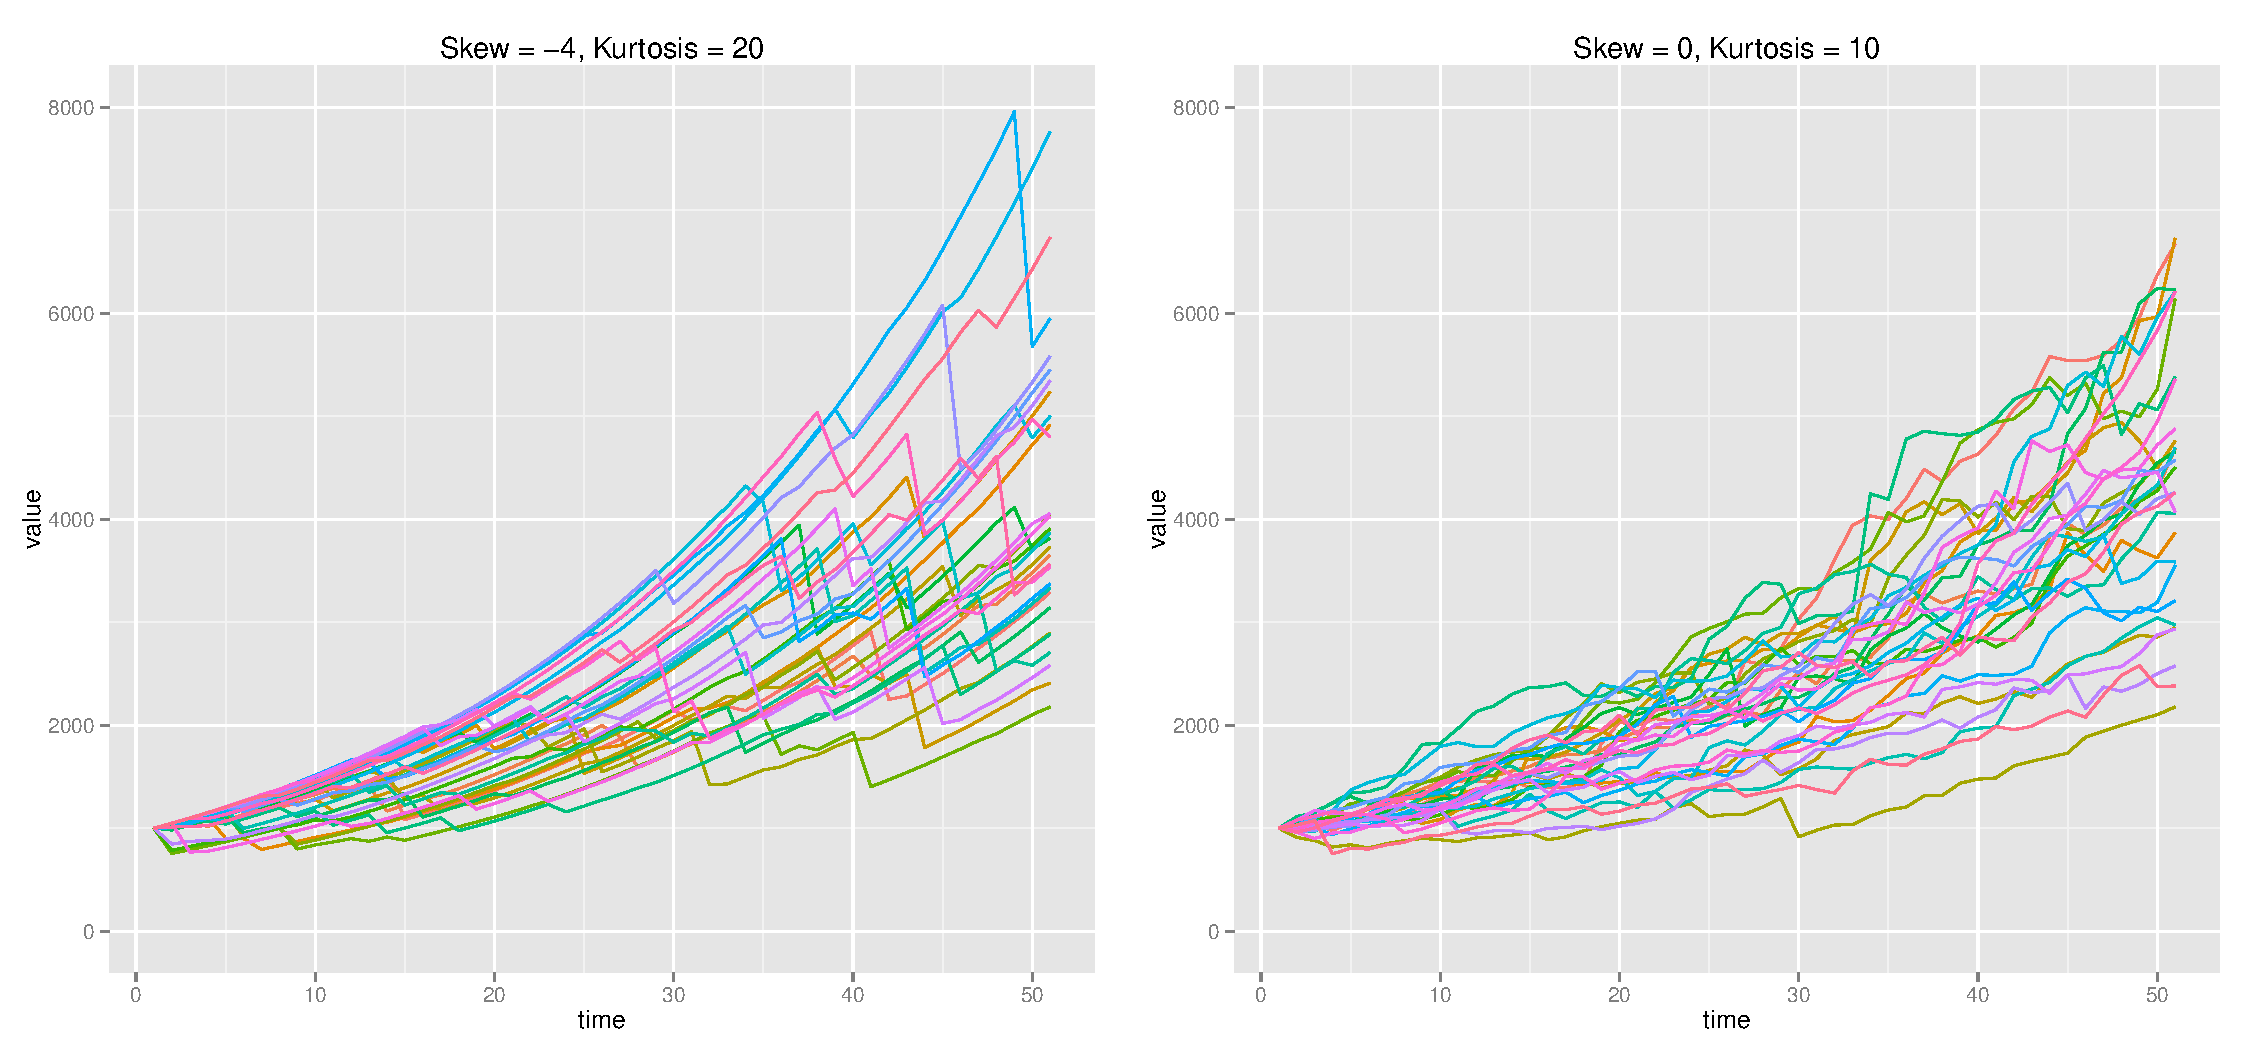
\includegraphics[width=4.5in]{plots/DVApaths2.pdf}
\caption{Sample Dollar Value Paths for Distributions with Mean 3 and Sigma 5}
\end{figure}
%\begin{figure}[H]
%\begin{minipage}[b]{4cm}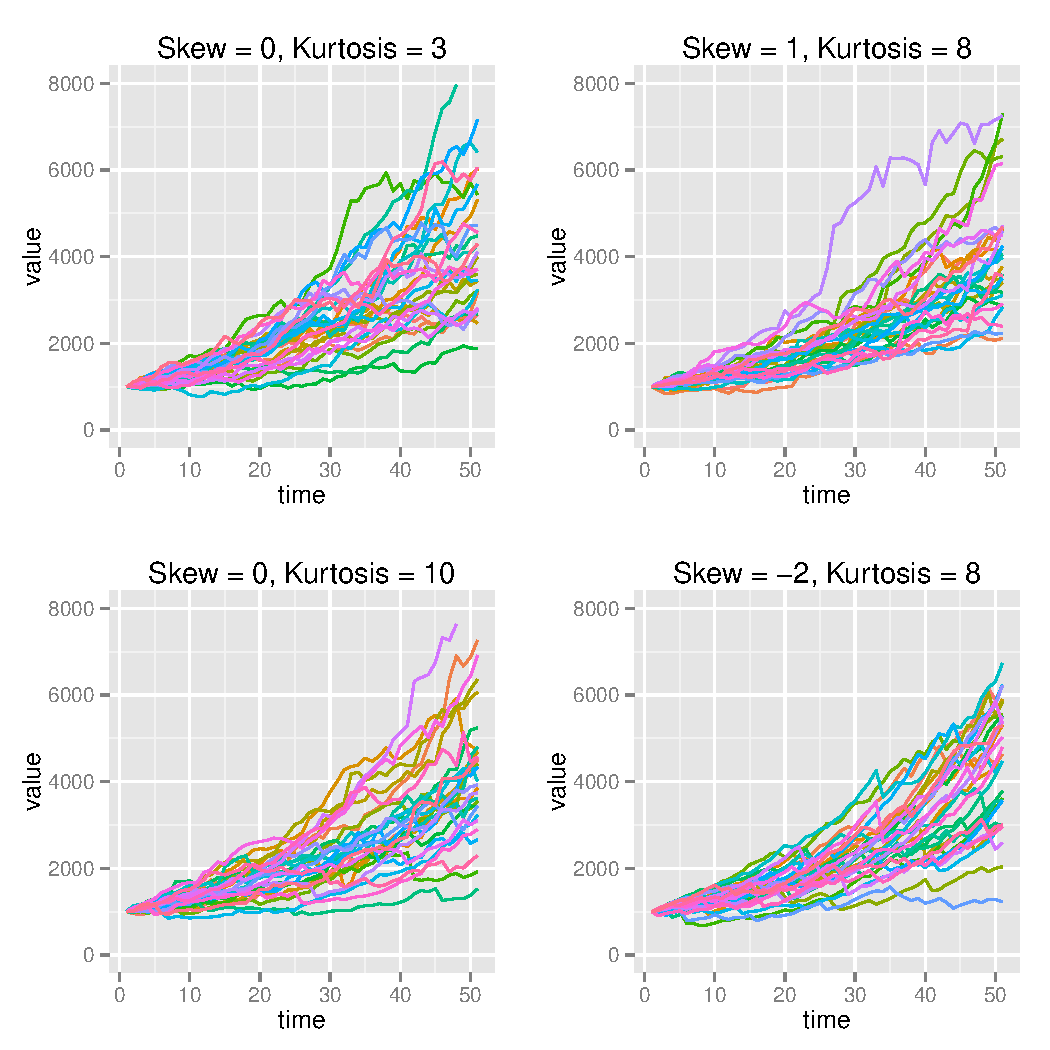
\includegraphics[4cm]{DVApaths.pdf}\end{minipage}
%\begin{minipage}{4cm}\caption{A nice figure}\end{minipage}
\end{frame}


\section{A Description of Omega}
\begin{frame}
Omega (also refered to as Gamma in the early literature)\cite{shadwick2002} is a performance measure defined as
\begin{align}
\Omega(L) = \dfrac{\int_L^b (1 - F(x))dx}{\int_a^L F(x)dx} \nonumber
\end{align}
where $L$ denotes the level at which we differentiate between a loss and a gain
\end{frame}

\begin{frame}
\underline{Pros}
\begin{itemize}
\item No parametric assumptions
\item Invariant under linear transformation:
\begin{align}
\varphi(x) 			&= ax + b \nonumber \\
\Omega(\varphi(L)) 	&= \Omega(L) \text{ if } a > 0 \nonumber \\
\Omega(\varphi(L)) 	&= \dfrac{1}{\Omega(L)} \text{ if } a < 0 \nonumber
\end{align}
\item $\dfrac{d\Omega}{dL} < 0$ everywhere and is as smooth as $F(L)$
\item Nice economic intuition, one can adjust the L depending on the state of macro-economy
\item Sub-additive
\end{itemize}
\end{frame}

\begin{frame}
\underline{Cons}
\begin{itemize}
\item $\Omega$ takes a value of 1 when $L = \mu$, i.e. does not distinguish between distribution with same mean at the mean point
\item Possibly unbounded given an infinite interval
\item Carries downside-type characteristic, so difficult to use if no sample returns are below the threshold
\end{itemize}
\end{frame}

\section{Simulation Methodology}

\begin{frame}
The Johnson family of distributions\cite{johnson1949} are a set of densities where the first four central moments can be specified given appropriate choice of parameters. They consists of continuous random variables $z$ such that when appropriately transformed become standard normal\cite{simonato2011}, i.e.
\begin{align}
y = a + b \times g(\dfrac{z-c}{d}), \hspace{4mm} y \sim N(0,1)
\label{eq:distribution}
\end{align} 

Where a and b in Equation (\ref{eq:distribution}) are shape parameters, c is a location parameter, d is a scale parameter and $g(\cdot)$ is one of the following four functions
\begin{align}
g(u) = 
\begin{cases}
\ln(u) \hspace{25mm} &\text{lognormal family}\\
\ln(u + \sqrt{u^2+1}) &\text{unbounded family}\\
\ln\big(\dfrac{u}{1-u}\big) &\text{bounded family}\\
u &\text{normal family}
\end{cases}
\label{eq:Cases}
\end{align}
\end{frame}

\begin{frame}
Given the first for moments, \citet{hill1976} discussed an algorithm for determining the associated Johnson family parameters. Denoting $S_L$, $S_U$ and $S_B$ as the lognormal, unbounded and bounded cases of Equation (\ref{eq:Cases}) respectively, the alorithm is as follows:
\vspace{3mm}

Letting $\sqrt{\beta_1} = \dfrac{\mu_3}{\sigma^3}$, $\beta_2 = \dfrac{\mu_4}{\sigma^4}$ and $\omega = e^{-b^2}$, first solve
\begin{align}
(\omega - 1)(\omega + 2)^2 = \beta_1 \nonumber
\end{align}
Then
\begin{align}
\beta_2 &< \omega^4 + 2\omega^3 + 3\omega^2 - 3 \Longrightarrow g(\cdot) = S_B \nonumber \\
\beta_2 &> \omega^4 + 2\omega^3 + 3\omega^2 - 3 \Longrightarrow g(\cdot) = S_U \nonumber \\
\beta_2 &= \omega^4 + 2\omega^3 + 3\omega^2 - 3 \Longrightarrow g(\cdot) = S_L \nonumber
\end{align}
\end{frame}

\begin{frame}
\underline{For $S_L$}
\begin{align}
b &= \ln(\omega)^{-{\frac{1}{2}}} &a& = \dfrac{1}{2}b\times \ln\Big(\dfrac{\omega (\omega -1)}{\sigma}\Big) \nonumber \\
c &= sign(\mu_3)\cdot\mu - e^{\frac{\frac{1}{2}b - a}{b}} &d& = sign(\mu_3) \nonumber
\end{align}

\underline{For $S_U$}\\
\vspace*{3mm}
If $\beta_1 = 0$
\begin{align}
\omega = [(2\beta_2 - 2 )^{\frac{1}{2}} - 1]^{\frac{1}{2}}, \hspace*{5mm} b = (\ln\omega)^{-\frac{1}{2}}, \hspace*{5mm} a = 0 \nonumber
\end{align}
If $\beta_1 \neq 0$
\begin{align}
\omega_1 = [(2\beta_2 - 2.8\beta_1 - 1)^{\frac{1}{2}} - 2]^{\frac{1}{2}} \nonumber
\end{align}
as an initial estimate and $\omega$, a and b are found using the \citet{johnson1969} iterative method 
\end{frame}

\begin{frame}
Then c and d are found using
\begin{align}
\sigma^2 &= \dfrac{1}{2}d^2(\omega - 1)(\omega cosh\Big(\dfrac{2a}{b}\Big) + 1) \nonumber \\
\mu 	 &= c - d\omega^{\frac{1}{2}}sinh\Big(\dfrac{a}{b}\Big) \nonumber
\end{align}

\underline{For $S_B$}
\vspace*{3mm}
\begin{align}
b &= \dfrac{0.626\beta_2 - 0.408}{(3 - \beta_2)^{0.479}} \hspace*{5mm} &\text{if } \beta_2 \geq 1.8 \nonumber \\
b &= 0.8(\beta_2 - 1) &\text{otherwise} \nonumber
\end{align}
Using \citet{draper1951}, $a$ is calculated. From initial estimates of $a$ and $b$ the first 6 moments are calculated using \citet{draper1952} and then Newton-Rhapson is used to solve for $a$ and $b$, and the first two moments are then used to determine $c$ and $d$

\end{frame}

\begin{frame}
Then we can simulate from the Johnson random variable using
\begin{align}
z = c + d \times g^{-1}\Big(\dfrac{y - a}{b}\Big)
\end{align}
with
\begin{align}
g^{-1}(u) = 
\begin{cases}
e^u \hspace{25mm} &\text{lognormal family}\\
(e^u - e^{-u})/2 &\text{unbounded family}\\
1/(1 + e^{-u}) &\text{bounded family}\\
u &\text{normal family}
\end{cases}
\end{align}
\end{frame}

\section{Distributional Effects on Omega}

\begin{frame}
\begin{figure}
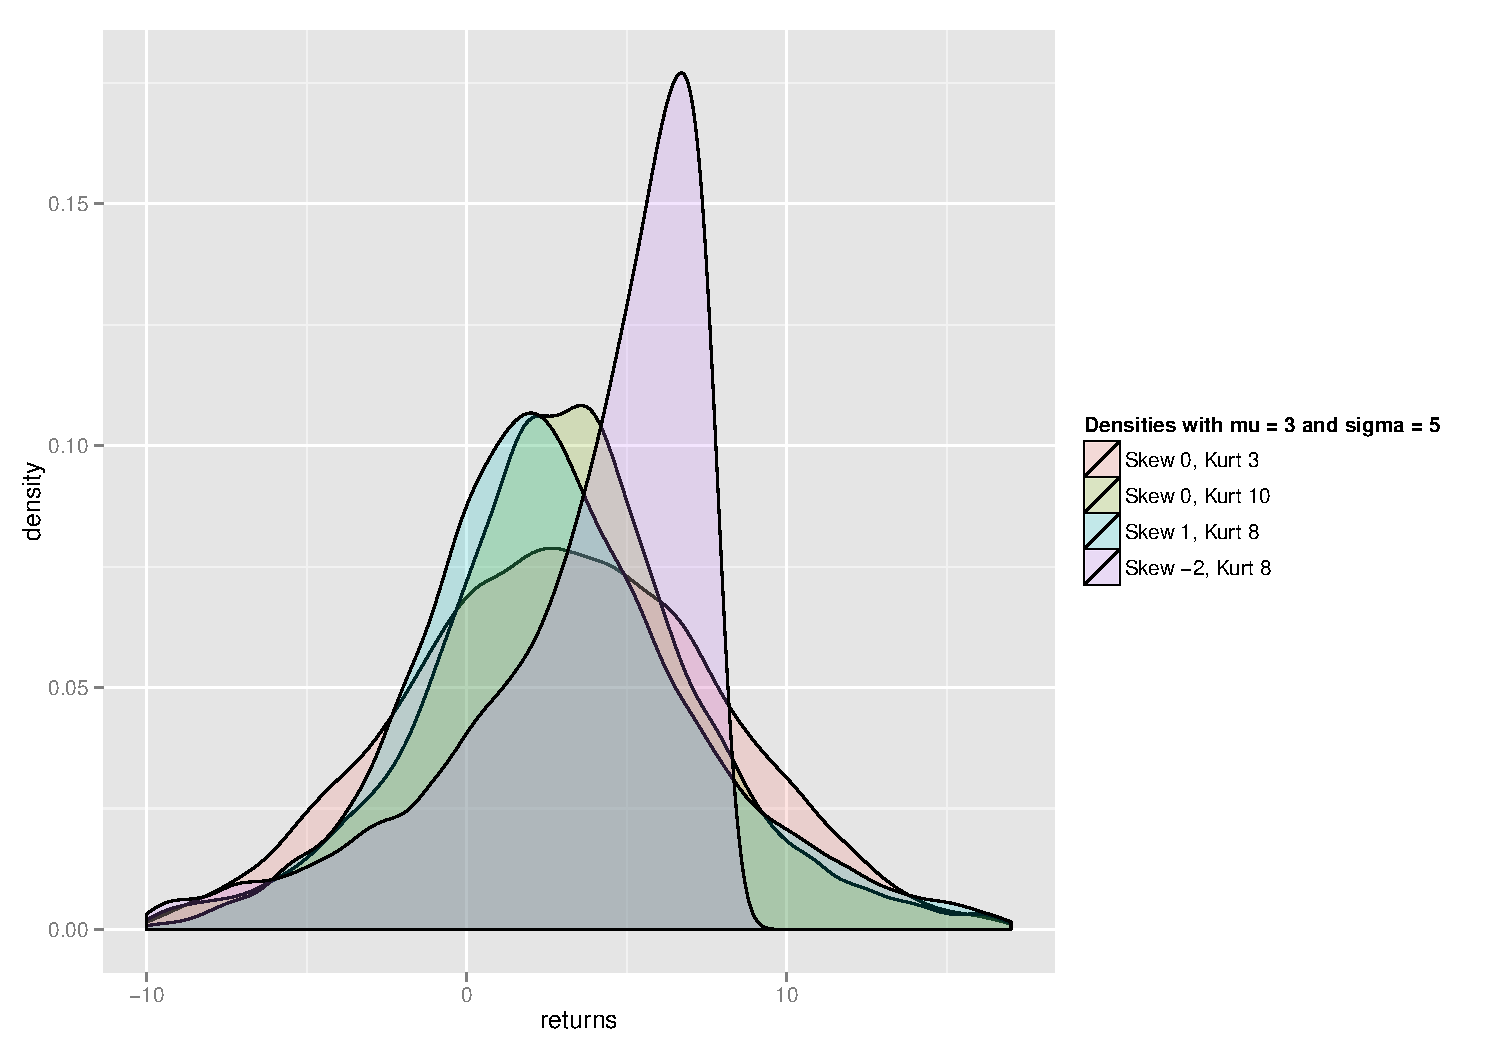
\includegraphics[width=3.75in]{plots/Densities.pdf}
\end{figure}
\end{frame}

\begin{frame}
\begin{figure}
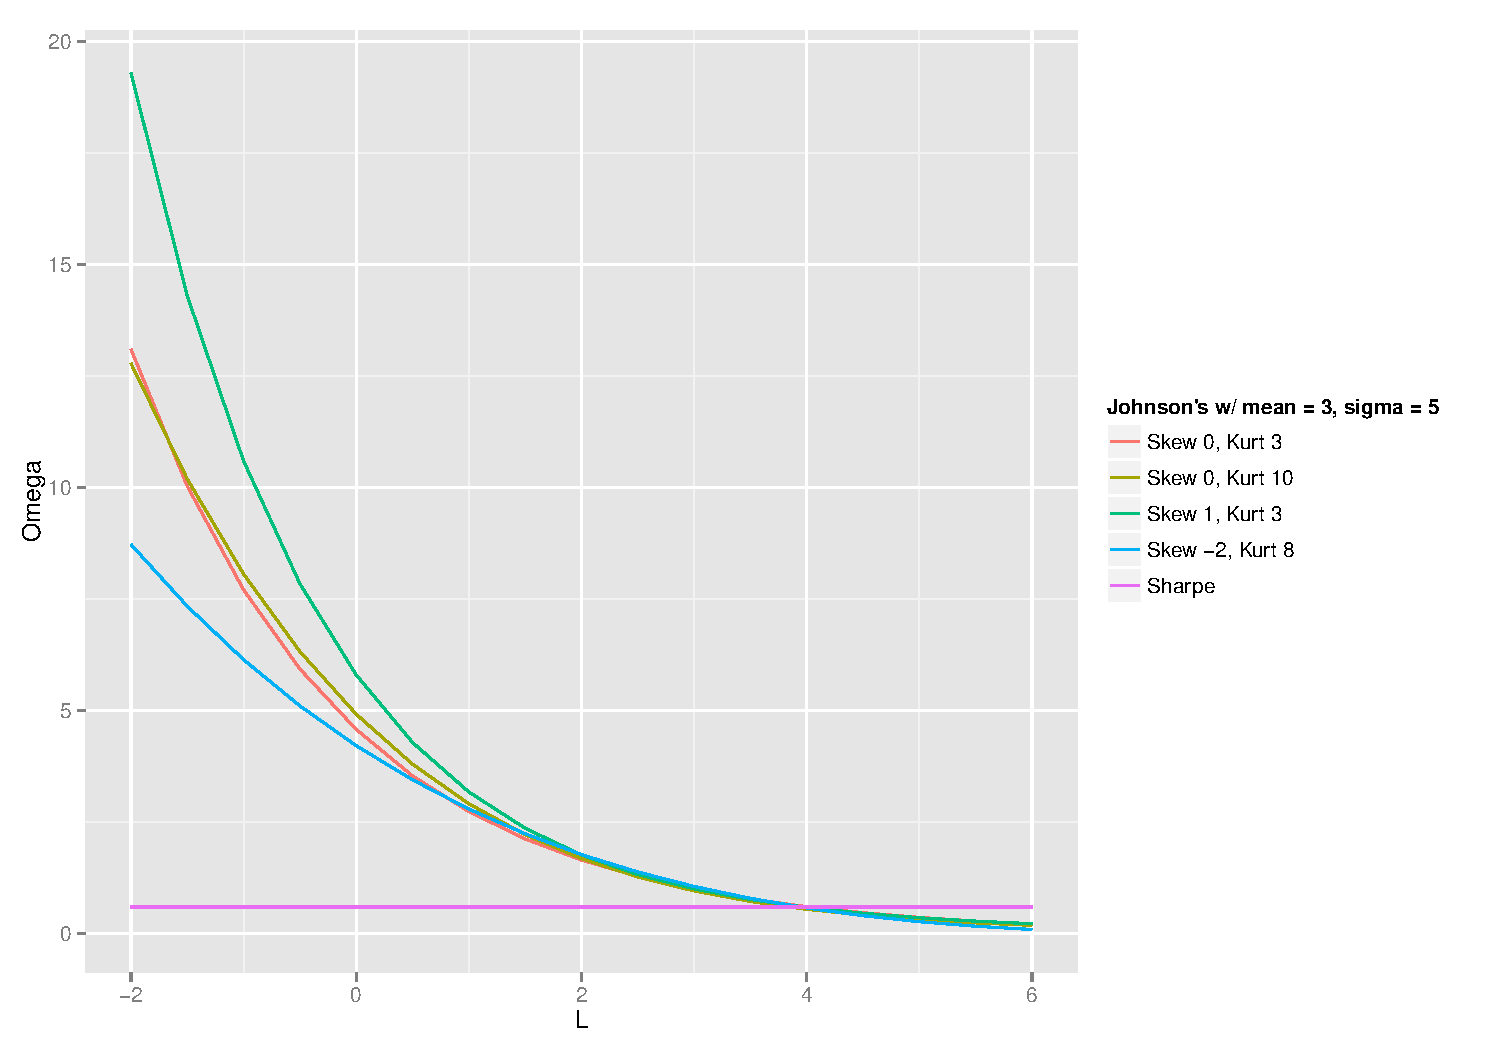
\includegraphics[width=3.75in]{plots/Preferences.pdf}
\end{figure}
\end{frame}

\section{An Empirical Study}

\begin{frame}
\begin{figure}
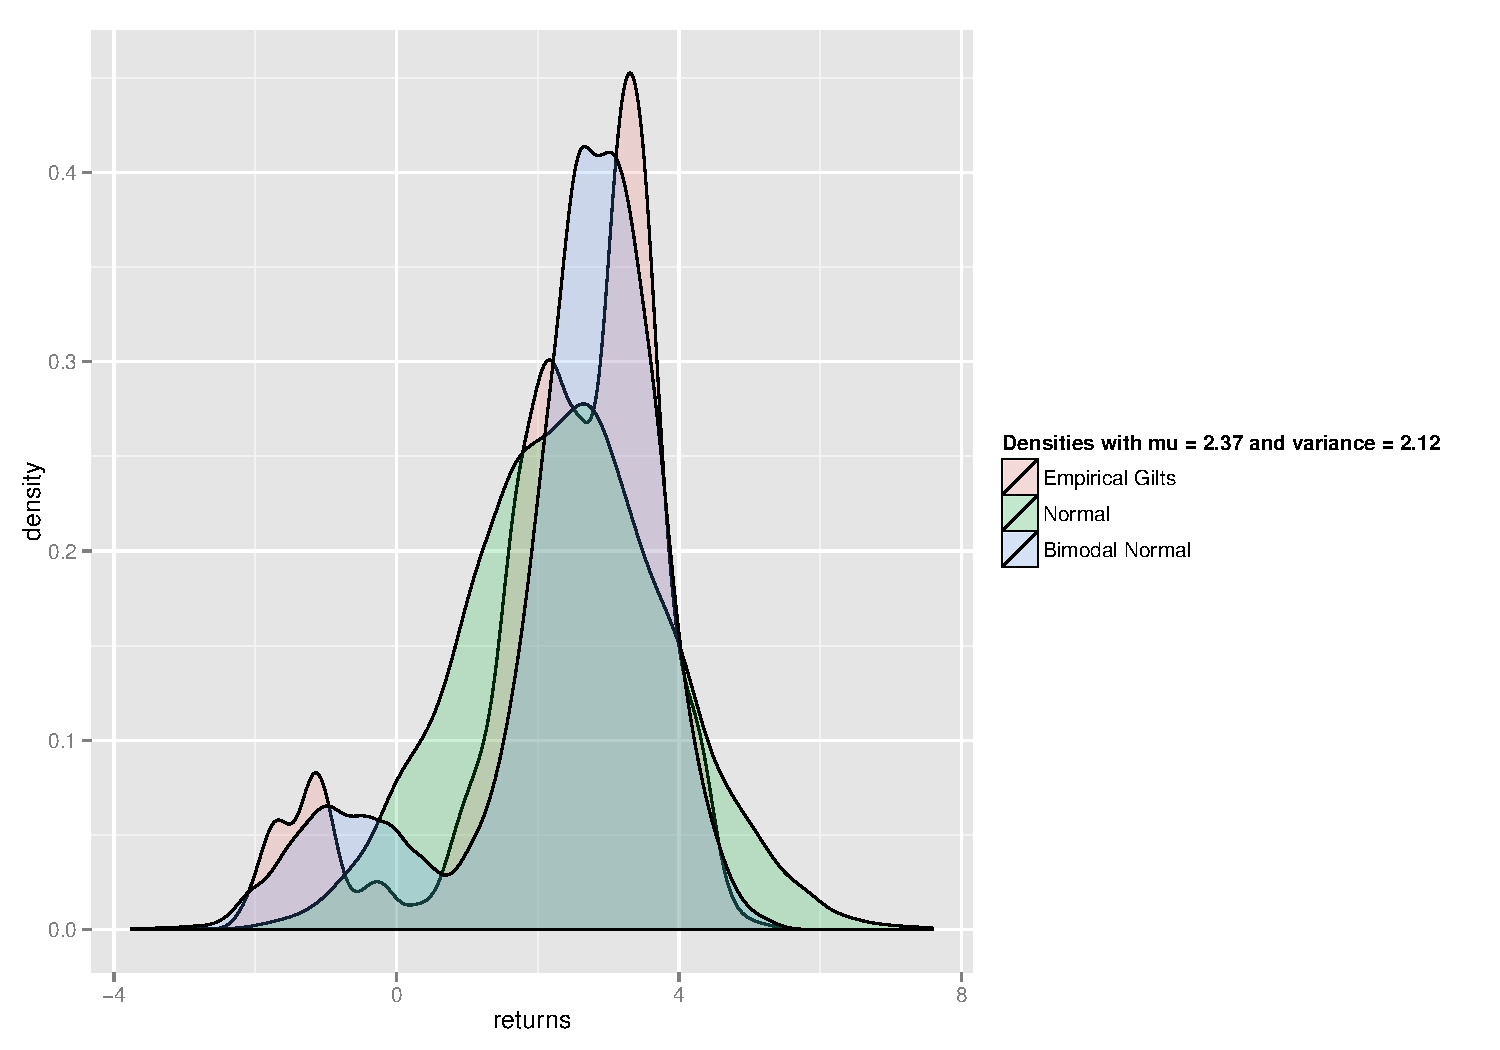
\includegraphics[width=3.75in]{plots/EmpiricalDensities.pdf}
\end{figure}
\end{frame}

\begin{frame}
\begin{figure}
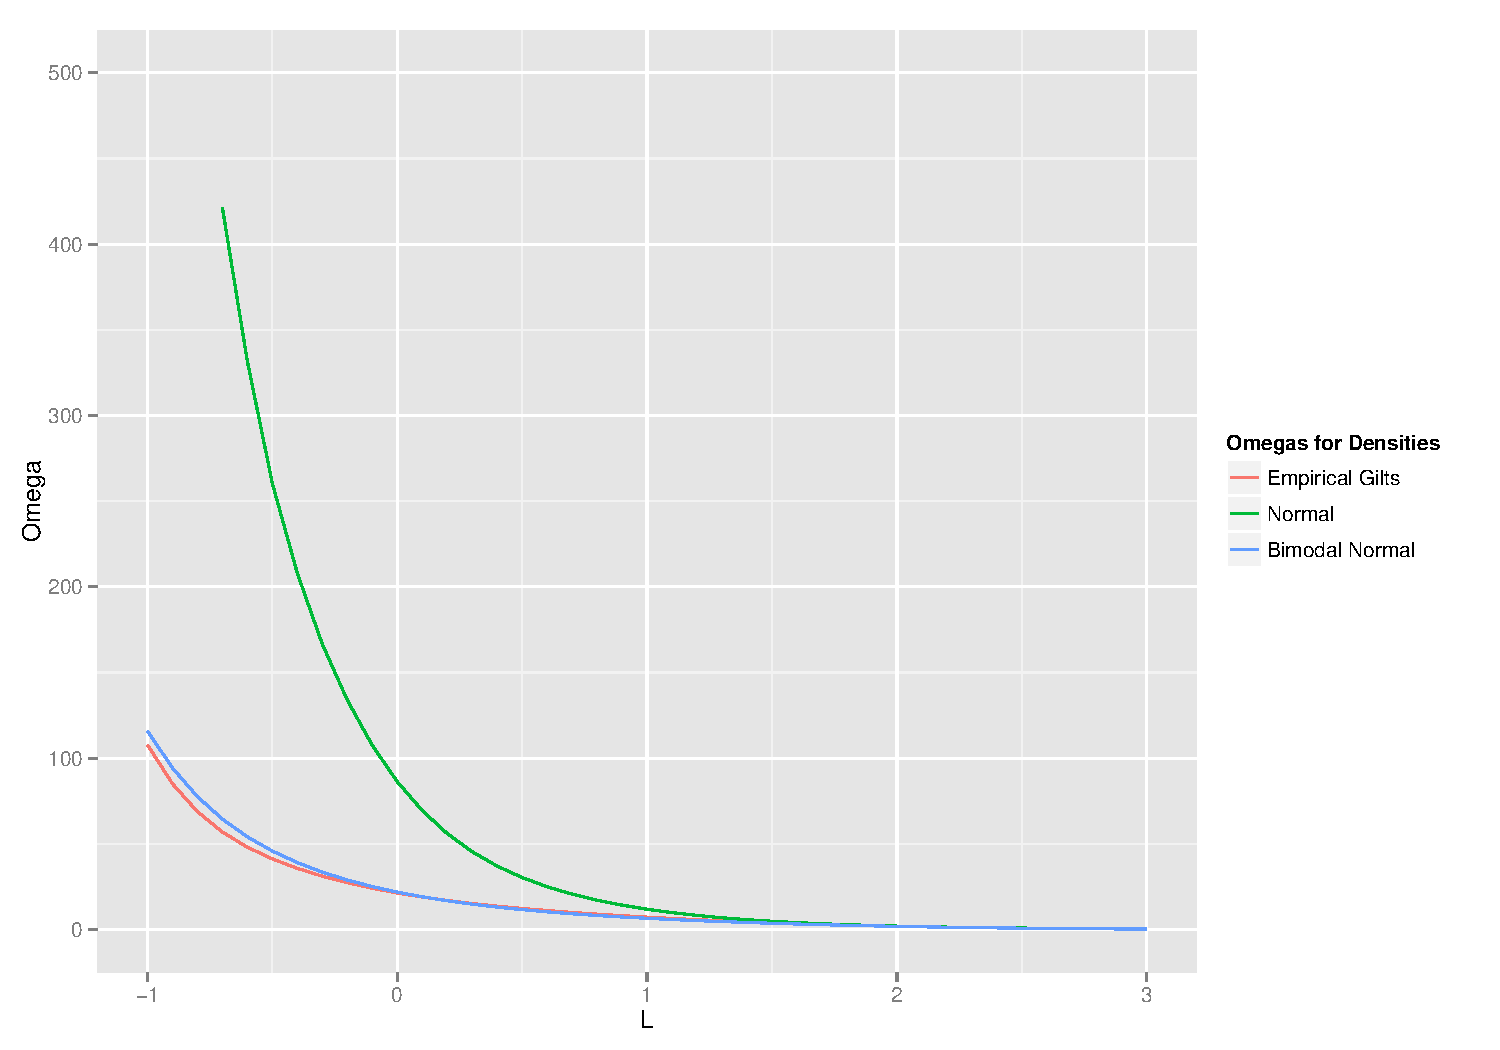
\includegraphics[width=3.75in]{plots/EmpiricalOmegas.pdf}
\end{figure}
\end{frame}


\section{Concluding Remarks and Future Work}
\begin{frame}
\begin{itemize}
\item The Omega performance measure provides a useful alternative to a Sharpe performance measure since it is well known financial returns are not normal and does not require a specific choice of utility
\item Investigate real world performance of hedge fund data using Sharpe and Omega
\item Determine the effects of sampling frequency on the estimation error of Omega
\end{itemize}
\end{frame}

\begin{frame}
    \bibliographystyle{abbrvnat}
    \bibliography{906References}
\end{frame}

%\begin{frame}
%\addcontentsline{toc}{section}{References}
%\bibliographystyle{apalike}
%\bibliography{906References}
%\end{frame}

\end{document}
